\documentclass[11pt]{article}
\usepackage[utf8]{inputenc}
\usepackage[T1]{fontenc}
\usepackage{amsmath}
\usepackage{amsfonts}
\usepackage{amssymb}
\usepackage[version=4]{mhchem}
\usepackage{stmaryrd}
\usepackage{graphicx}
\usepackage[export]{adjustbox}
\graphicspath{ {./images/} }
\usepackage{hyperref}
\hypersetup{colorlinks=true, linkcolor=blue, filecolor=magenta, urlcolor=cyan,}
\urlstyle{same}

\begin{document}
Leveraged Buyouts (LBOs)

A buyout is described as an LBO when, after the buyout, the debt-to-equity ratio is much greater than before the acquisition. In fact, the debt-to-equity ratio can be as high as 9:1, meaning the capital structure of the company after the buyout is $90 \%$ debt and 10\% equity. An LBO typically includes an effort to make fundamental changes in the management and/or operations of the target.

\section*{History of Leveraged Buyouts}
Although buyouts began after World War II, it was not until the 1970s that their investment value became apparent. In 1976, a new investment firm, Kohlberg Kravis Roberts \& Co. (KKR), was created on Wall Street with just \$3 million of its own funds to invest. The founders of KKR had previously worked at Bear Stearns Companies, where they helped pioneer buyout transactions as early as 1968. No firm has had a greater impact on the buyout market than KKR, which has conducted landmark transactions, such as the buyout of RJR Nabisco.

The 1980s witnessed the rise of a key element of the growth in buyouts: financing of the buyouts using bonds with low credit ratings, known as junk bonds. Junk bonds are debt instruments with high credit risk, also referred to as high-yield, non-investment-grade, or speculative-grade debt. Bonds with low credit ratings previously existed, primarily as a result of a decline from an initial investment-grade rating. Michael Milken of Drexel Burnham Lambert helped pioneer the use of high-yield debt as a financing tool by issuing junk bonds to finance buyouts.

Fueled by junk bond financing, buyout deals reached an initial peak in 1989, when KKR bought the giant food conglomerate RJR Nabisco Inc. for $\$ 31$ billion in a deal that was documented in the book and movie Barbarians at the Gate. ${ }^{1}$ Bryan Burrough and John Helyar, Barbarians at the Gate: The Fall of RJR Nabisco (New York: Harper \& Row, 1990). This buyout would stand as the largest buyout for many years, until KKR surpassed the RJR Nabisco deal in 2006 with its bid for TXU Corporation, a major Texas-based utility company. The subsequent large debt load of Energy Future Holdings, the holding company successor to TXU, led to its bankruptcy in 2014. The bankruptcy is also attributed to the company's heavy reliance on coal-fired generation facilities, which struggled to compete with natural gas power production due to the depressed prices of natural gas and the increased supply of natural gas from improved production techniques (e.g., fracking).

In the 1990s, buyout activity declined for two reasons. First, the recession of 1990-91, that affected most major world economies, briefly pushed credit spreads to high levels and thus dampened the attractiveness of junk bond financing for buyouts. Second, in 1998, the Russian government defaulted on its sovereign bonds, which once again sent credit spreads spiraling upward. Whereas debt represented as much as $95 \%$ of the financing of some buyout deals during the 1980 s, by the end of the 1990 s, buyouts financed with more than $75 \%$ debt were viewed as unattractive.

Bain publishes an annual Global Private Equity Report that in 2022 reported global buyout deal values and numbers as reproduced in the exhibit Global Buyout Deal Values and Counts. As evidenced in the exhibit below, the new millennium started quietly for the buyout market, but availability of credit increased in the United States and elsewhere, leading to an unparalleled boom in buyouts from 2003 into early 2007 . This buyout boom culminated in the largest buyout ever: the $\$ 45$ billion buyout of TXU Corporation. But by late 2007, the liquidity bubble had burst, leading to the credit problems of 2008 and the swift decline of buyout activity. Thus, buyout activity is driven not just by economic growth but also by interest rates and credit spreads. Note that in the 10 years subsequent to the global financial crisis, deal sizes and counts have resumed growth but have yet to reach the pre-crisis levels of 2006 and 2007.

\begin{center}
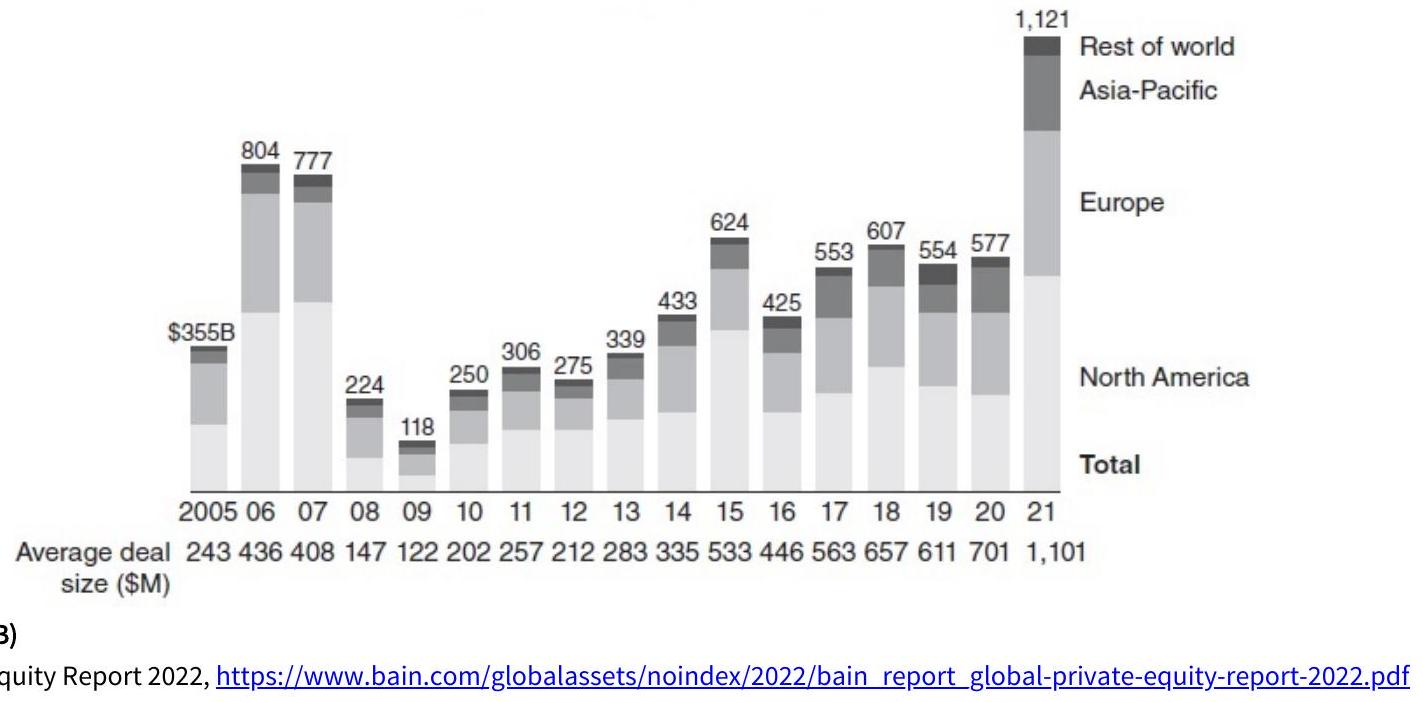
\includegraphics[max width=\textwidth]{2024_04_10_9c5a16d2bfd1e32f16c8g-2}
\end{center}

Global Buyout Deal Values (\$B)

Source: Bain Global Private Equity Report 2022, \href{https://www.bain.com/globalassets/noindex/2022/bain}{https://www.bain.com/globalassets/noindex/2022/bain} report global-private-equity-report-2022.pdf

\section*{Three Key Economic and Agency Issues of Buyouts}
Three economic and agency issues related to buyouts are key:

\section*{Are Buyout Markets Segmented and Informationally Inefficient?}
Buyout activity was previously thought to take place in a segmented market. Segmentation, in this context, denotes the grouping of market participants into clienteles that focus their activities within specific areas of the market, rather than varying their range of activities more broadly throughout all available opportunities. When a market is segmented, the valuations in that market can vary based on the preferences of the clienteles that dominate the particular segments. For example, it is often argued that the fixed-income market is segmented, based on the maturity ranges in which different investors (clienteles) prefer to invest. Thus, short-term yields might be argued to be driven by money market investors, whereas longer-term yields are driven by pension and insurance firms in a segmented market.

Buyout activity was also previously thought to take place in an inefficient market. Inefficiency refers to informational inefficiency, the idea that transactions take place with relatively large divergences between the actual prices of the transactions and the true underlying values of those transactions, based on all available information. Segmentation can lead to informational market inefficiency.

An evolution of the buyout market has occurred that has been driven by substantial buyout activity and has resulted in a less segmented market that has grown into a more efficient, auction-driven asset market, in which greater competition has reduced abnormal profit opportunities.

Are Management Buyouts a Violation of Fiduciary Duties?

Buyouts can have large economic consequences to both the managers and shareholders of the target firm. There is an inherent conflict of interest between the shareholders as principals and the managers as agents with regard to most buyouts. That conflict of interest can become especially important in the high-stakes environment of buyouts. The primary conflicts involved in management buyouts are quite distinct from the conflicts involved in management buy-ins.

In an MBO, the existing management team takes over ownership of the firm from the firm's existing shareholders.

Managers clearly owe a fiduciary duty to the shareholders of the firm in which they are employed. Managers tend to have superior information regarding the firm and its potential value. Presumably, in a management buyout, the incumbent managers perceive that there are substantial gains that can be unlocked through their actions. A critical issue is whether managers choosing to pursue a path of unlocking those gains through a management buyout are violating their fiduciary responsibilities to the firm's shareholders. In other words, if a management team leads a buyout that unlocks tremendous value for themselves rather than implementing those changes for the firm's existing owners, has the management team as agents enriched themselves at the expense of the principals? Or do the existing shareholders receive a generous sales price based on the anticipated benefits that the new management team will be able to unlock after the buyoutbenefits that could not be unlocked under the current ownership structure and incentives? In the latter case, the managers might be best fulfilling their fiduciary responsibility by initiating an MBO.

\section*{Are Managers Perversely Incentivized with Regard to Management Buyins?}
In an MBI, an external management team replaces the existing management team. The outcome of an MBI for incumbent managers can vary tremendously depending on the extent to which the managers are compensated upon their departure.

A generous compensation scheme, known as a golden parachute, is often given to top managers whose careers are being negatively affected by a corporate reorganization. Two primary conflicts of interest emanate from these potentially lucrative compensation schemes. First, incumbent managers have a strong incentive to resist any buyout attempt (no matter how lucrative to shareholders) that displaces them as managers if the buyout does not provide them with generous compensation. Second, incumbent managers have a strong incentive to encourage buyouts that offer them generous compensation. Thus, incumbent managers are incentivized to interfere with buyouts or promote buyouts based on the financial implications to themselves rather than based purely on their duties to serve the interests of the shareholders.

\section*{Five General Categories of LBOs That Can Create Value}
Most LBOs can be identified with one of five major categories based on the motivation or circumstances of the deal.

\begin{enumerate}
  \item Efficiency buyouts: Efficiency buyouts are LBOs that improve operating efficiency. A company may be bought out because it is shackled with a noncompetitive operating structure. For large public companies with widespread equity ownership, management may have little incentive to create shareholder value because it has a small stake in the company's profit. Under these circumstances, management is likely to be compensated based on revenue growth, which may result in excessive expansion and operating inefficiencies. These examples often occur in mature industries with stable cash flows.
\end{enumerate}

Efficiency buyouts often lead to a reduction in firm assets and revenue with the goal of eventually increasing firm profits. Such a buyout introduces more concentrated ownership and a better incentive scheme to mitigate agency problems. Management is given a stake in the company with an incentive scheme tied not to increasing revenues but to increasing operating margins and equity value. In addition, a high leverage ratio is used to ensure that management has little discretion to invest in inefficient projects. Last, the LBO firm replaces the diverse shareholder base and provides the active oversight that was lacking with the prior widespread equity owners.

\begin{enumerate}
  \setcounter{enumi}{1}
  \item Entrepreneurship stimulators: Entrepreneurship stimulators are LBOs that create value by helping to free management to concentrate on innovations. One frequently used strategy focuses on an unwanted or neglected operating division. Often an operating division of a conglomerate is chained to its parent company, which may impede its ability to implement an effective business plan. An LBO can free the operating division to control its own destiny.

  \item The overstuffed corporation: One of the main targets of many LBO firms is conglomerates. Conglomerates have many different divisions or subsidiaries, often operating in completely different industries. Wall Street analysts are often reluctant to follow or cover conglomerates because they do not fit neatly into any one industrial category. As a result, these companies can be misunderstood by the investing public and perhaps undervalued. Sometimes conglomerates drain profits from profitable divisions within the firm and use them to prop up failing divisions rather than reinvesting them in successful divisions or distributing them to shareholders as dividends. An LBO can be used to dismantle inefficient conglomerates, shut down or sell inefficient operations, and allow profitable divisions to reinvest and meet their growth potential.

  \item Buy-and-build strategy: A buy-and-build strategy is an LBO value-creation strategy involving the synergistic combination of several operating companies or divisions through additional buyouts. The LBO firm begins with one buyout and then acquires more companies and divisions that are strategically aligned with the initial LBO portfolio company. The strategy seeks to benefit from synergies realized through the combination of several different companies into one. In some respects, this strategy is the reverse of that for conglomerates. Rather than strip a conglomerate down to its most profitable divisions, this strategy pursues an assembling approach. This type of strategy is also known as a leveraged buildup or roll up.

  \item Turnaround strategy: Traditional buyout firms often look for successful, mature companies with low debt-to-equity ratios and stable management. The economic recession that began in 2007 highlighted another form of LBO: the turnaround LBO. A turnaround strategy is an approach used by LBO funds that look for underperforming companies with excessive leverage or poor management. The targets for turnaround LBO specialists come from two primary sources: (1) ailing companies on the brink of bankruptcy, and (2) underperforming companies in another LBO fund's portfolio. In some cases, the private equity firm does not buy out the complete company but makes a large equity contribution at a price discounted to the public market price of the stock and takes seats on the target company's board of directors.

\end{enumerate}

\section*{The Appeal and Four Benefits of a Leveraged Buyout to Targets}
Leveraged buyouts can have a number of appealing characteristics to corporate management and investors of the target firm. From the perspective of the shareholders of the target firm, LBO offers are usually accepted because the bid price for their shares is typically at a large premium compared to the market price.

More to the point, LBO firms often target companies that have a depressed stock price. Consequently, shareholders often welcome an LBO bid. From the perspective of the target firm's corporate management, the benefits to those who are retained can include the following:

\begin{enumerate}
  \item The use of leverage where interest payments are tax deductible

  \item Less scrutiny from public equity investors and regulators

  \item Freedom from a distracted (and potentially distracting) corporate parent

  \item The potential of company management to become substantial equity holders and thereby benefit directly from building the business

\end{enumerate}

The benefit of an LBO to the acquiring LBO investor is the potential for attractive risk-adjusted returns. The following section provides a simplified example of the profit potential from a successful LBO.

\section*{Valuation of an LBO}
The potential payoffs of an LBO are like a call option: large upside potential relative to downside risk. Consider a publicly traded firm that is viewed by a private equity firm as a potential target, since it is failing to use its potential to generate earnings. The company has equity with a market value of $\$ 500$ million and debt with a face value of $\$ 100$ million. The company is currently generating earnings before interest, taxes, depreciation, and amortization (EBITDA) of $\$ 80$ million, which represents the free cash flow from operations that is available for the owners and debtors of the company. This equates to a $13.3 \%$ before-tax return on assets for the company's shareholders and debt holders.

An LBO fund uses $\$ 700$ million to purchase the equity of the company and pay off the outstanding debt. The debt is paid off at a face value of $\$ 100$ million, while the remaining $\$ 600$ million is offered to the equity holders to entice them to tender their shares to the LBO fund (i.e., a $20 \%$ premium is offered over the current market value). The $\$ 700$ million LBO is financed by the LBO fund with $\$ 600$ million in debt at a $10 \%$ coupon rate and $\$ 100$ million in equity. Thus, the company must pay $\$ 60$ million in annual debt service to meet its interest payment obligations. (The debt load in this example is not realistic, but used for illustration only, as buyouts in 2017 had average equity contributions of five times equity and six times debt for a debt-to-enterprise value ratio of $54.5 \%$.)

After the LBO, the management of the company improves operations, streamlines expenses, and implements better asset utilization. One explanation for the improved managerial performance might be that the LBO fund brought in new management. Another possibility is that some or all of the existing top management initiated the LBO and became highly incentivized to improve profitability. As a result, assume that the cash flow from operations of the company improves from $\$ 80$ million to $\$ 120$ million per year. By forgoing dividends and using the free cash flow to pay down the remaining debt, the LBO fund can own the target company free and clear of the debt used to finance the acquisition in about seven years. This means that after seven years and ignoring potential growth in cash flows, the LBO firm as the sole equity owner can claim the annual cash flow of $\$ 120$ million completely for itself.

After the seven-year point, assume a forward-looking long-term growth rate of $2 \%$ per year and a discount rate of $12 \%$. The value of the unlevered firm in seven years can be projected using the constant dividend growth model, as follows:

$$
\$ 120 \text { million } /(0.12-0.02)=\$ 1.2 \text { billion }
$$

Under these assumptions, the LBO fund can own the $\$ 1.2$ billion company free and clear in seven years, starting with an equity investment of only $\$ 100$ million. The total return on the investment for the LBO transaction would be as follows:

$$
(\$ 1.2 \text { billion } / \$ 100 \text { million })^{1 / 7}-1=42.6 \%
$$

The total return of $42.6 \%$ represents the annual compounded return on the equity portion of the LBO fund's investment. Notice the impact that leverage has on this transaction. The company is financed with a 6:1 debt-to-equity ratio. This is a very high leverage ratio for any company. The cash flows generated by the company were used to pay down the debt to a point where the company is completely owned by the equity holders. The equity holders receive a very high return because the debt used to finance the transaction is locked in at a $10 \%$ coupon rate. This means that most operating efficiencies and capital gains generated from the business accrue to the benefit of the equity holders - a keen incentive for equity holders to improve the operations of the company.

Notice that the total return to the leveraged equity investment is $42.6 \%$, far greater than the $8 \%$ unlevered return found as:

$(\$ 1.2 \text { billion } / \$ 700 \text { million })^{1 / 7}-1=8 \%$

The larger the leverage multiple, the larger the difference between the levered and unlevered return to equity.

Note that the numerator of the constant dividend growth model is the cash flow that is anticipated one year beyond the valuation date. Thus, if the valuation is being performed in year 7 , the cash flow that should be used as the numerator in the dividend growth model is the cash flow anticipated in year 8 . Often this is expressed as the year 7 cash flow multiplied by $(1+g)$, where $g$ is the projected annual growth rate. This aspect is introduced in the following application.

These applications illustrated a simplified LBO as being financed with a combination of debt and equity, with debt being the large majority of the financing. Generally in LBO deals there are three tranches of financing: senior debt, mezzanine debt, and equity. Senior debt typically entails financing from banks, credit/finance companies, insurance companies, or public debt offerings. Mezzanine debt is purchased by mezzanine debt funds (another form of private equity to be discussed in the session Private Credit and Distressed Debt), insurance companies, and other institutional investors. Last is the equity tranche, held by the LBO firm that has taken the company private, and it often includes some form of equity kicker for the mezzanine debt tranche.

\section*{Four Spillovers of Corporate Governance to the Public Market}
The principles of corporate governance that LBO firms apply to their private companies have four important benefits for the public market.

First, the strong governance principles that an LBO implements in its private firms should remain when those firms are taken public again. Second, LBO transactions serve as a warning to the management team of other public companies: If a company has a poor incentive scheme and minimal shareholder monitoring, it may be ripe for an LBO acquisition. Third, the incentive and monitoring schemes implemented by LBO firms for their portfolio companies provide guidance to managers and shareholders of other firms searching for more efficient governance methods. Last, as indicated earlier, conglomerates can be popular targets for LBO firms, and this can help stop unnecessary and inefficient diversification of large corporations.


\end{document}